%============================================================================
\section{Resultados y análisis}\label{sec:resultados}
%============================================================================

\subsection{Validación del enlace (prueba A)}\label{subsec:validacion}

En la referencia, la componente I alternó entre $\pm1$ con el leve
ensanchamiento del AWGN y Q contuvo solo ruido (Fig.~\ref{fig:tiempo_psd}a). La
PSD mostró el lóbulo principal centrado en $f=0$ y lóbulos laterales
decrecientes (Fig.~\ref{fig:tiempo_psd}e). El ojo presentó rampas lineales,
propias del integrador, con vértices en $\pm1$ cada \SI{31,25}{\micro\second}
(Fig.~\ref{fig:ojo_const}a), es decir, una apertura vertical de 2 en el
instante de decisión. Las nubes de la constelación sobremuestreada
($\approx\pm0{,}2$, Fig.~\ref{fig:const_sobre}a) se redujeron a
$\approx\pm0{,}07$ en la de decisión (Fig.~\ref{fig:ojo_const}e): el factor
$\sqrt8$ es la ganancia del filtro acoplado. La BER fue cero, lo que validó el
receptor y la alineación de los bits.

\subsection{Señal temporal y PSD}\label{subsec:res_tiempo_psd}

En D aparecieron cuatro picos, cerca de \num{1,5}, \num{3,45}, \num{5,4} y
\SI{7,35}{\milli\second}, separados unos \SI{1,95}{\milli\second} como en el
diseño ($N_T/f_s=\SI{1,953}{\milli\second}$), con alturas $1+A_i=5$ sobre símbolos $+1$ y $-1+A_i=3$ sobre $-1$
(Fig.~\ref{fig:tiempo_psd}d). En B y C solo fueron evidentes los impulsos sobre
símbolos $+1$; sobre un $-1$ llevaron la señal a 0 o a $+1$ durante
\SI{15,6}{\micro\second} y se confundieron con una transición normal: una
perturbación de este nivel puede imitar un símbolo válido. Q no se alteró,
porque el impulso es real. Las cuatro PSD conservaron la misma forma, con
diferencias del orden de las fluctuaciones de cada captura
(Fig.~\ref{fig:tiempo_psd}e--h). Con $\delta=0{,}008$ la potencia media del
impulso es baja y se reparte en una banda ancha, de modo que la PSD, una medida
promediada, resultó poco sensible a esta perturbación escasa e intensa, a diferencia del
AWGN, que eleva el piso espectral de forma visible~\cite{middleton1977,pighi2009}.

\subsection{Constelación y diagrama de ojo}\label{subsec:res_const_ojo}

En la constelación sobremuestreada aparecieron pocos puntos desplazados
exactamente $A_i$: en 0 y 2 (B), 1 y 3 (C), y 3 y 5 (D)
(Fig.~\ref{fig:const_sobre}b--d), pues solo 4 de cada 500 muestras están
perturbadas. En la de decisión el desplazamiento fue la mitad: $-0{,}5$ y
$1{,}5$ (B), 0 y 2 (C), y $+1$ y 3 (D) (Fig.~\ref{fig:ojo_const}f--h), lo que
confirma $A_{\mathrm{ef}}=A_i/2$. En C, los símbolos $-1$ alcanzados quedaron
sobre el umbral; en D se superpusieron a la nube de $+1$ y se decidieron mal. En
el ojo, la mayoría de los trazos no cambió y el margen de los $-1$ alcanzados,
$1-A_{\mathrm{ef}}$, pasó de 1 a $0{,}5$, 0 y $-1$ en B, C y D
(Fig.~\ref{fig:ojo_const}b--d): el cierre no fue uniforme, como con AWGN, sino
limitado al $1{,}6\,\%$ de símbolos afectados.

\subsection{Tasa de error de bit}\label{subsec:res_ber}

\begin{table}[!t]
\centering
\caption{BER medida frente a la BER teórica de~\eqref{eq:pb_imp}, con bits
equiprobables ($p_-=1/2$) y con la secuencia periódica empleada ($p_-=11/16$)}
\label{tab:ber}
\footnotesize
\setlength{\tabcolsep}{3.5pt}
\begin{tabular}{@{}cccccc@{}}
\toprule
\textbf{Prueba} & \textbf{$A_i$} & \textbf{$1-A_{\mathrm{ef}}$} &
\textbf{$p_-=1/2$} & \textbf{$p_-=11/16$} & \textbf{Medida} \\
\midrule
A & 0   & 1   & 0                    & 0                    & 0 \\
B & 1,0 & 0,5 & $\approx 0$          & $\approx 0$          & 0 \\
--& 1,8 & 0,1 & $2{,}5\times10^{-7}$ & $3{,}5\times10^{-7}$ & 0 \\
--& 1,9 & 0,05& $1{,}8\times10^{-4}$ & $2{,}5\times10^{-4}$ & $2{,}8\times10^{-4}$ \\
C & 2,0 & 0   & $4{,}0\times10^{-3}$ & $5{,}5\times10^{-3}$ & $5{,}82\times10^{-3}$ \\
--& 2,1 & $-0{,}05$ & $7{,}8\times10^{-3}$ & $1{,}07\times10^{-2}$ & $1{,}07\times10^{-2}$ \\
D & 4,0 & $-1$ & $8{,}0\times10^{-3}$ & $1{,}10\times10^{-2}$ & $1{,}10\times10^{-2}$ \\
\bottomrule
\multicolumn{6}{@{}p{0.95\columnwidth}@{}}{\scriptsize Para $A_i=0{,}5$ y
$1{,}5$ la BER medida fue 0; para $A_i=2{,}2$, $2{,}5$, 3 y 5 fue
$1{,}1\times10^{-2}$.}
\end{tabular}
\end{table}

\begin{figure}[!t]
\centering
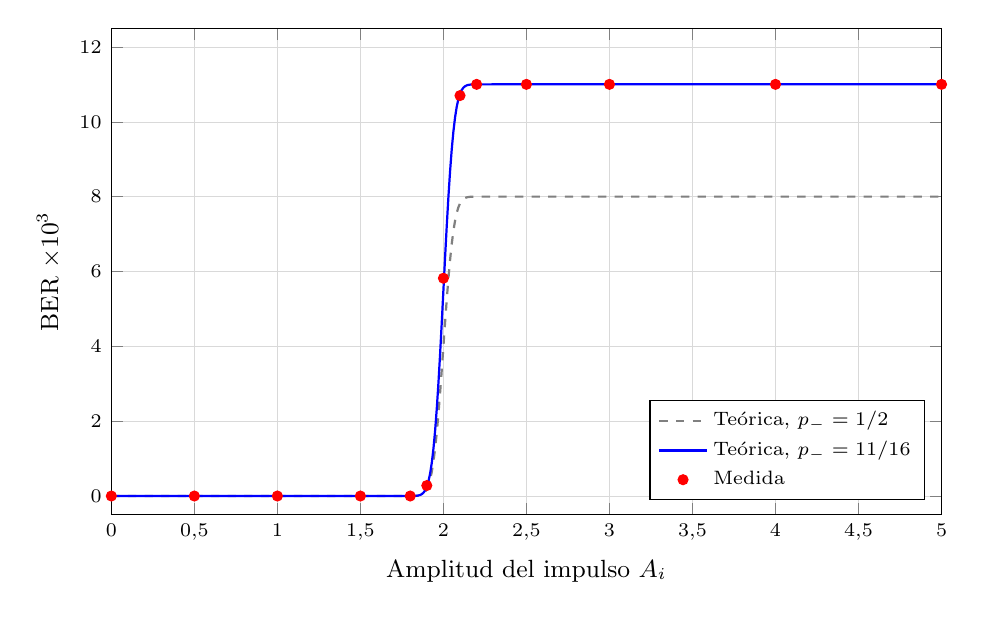
\begin{tikzpicture}
\begin{axis}[
  width=\columnwidth, height=0.64\columnwidth,
  xlabel={Amplitud del impulso $A_i$},
  ylabel={BER $\times 10^{3}$},
  xmin=0, xmax=5, ymin=-0.5, ymax=12.5,
  grid=both, grid style={line width=0.1pt, draw=gray!30},
  legend style={font=\scriptsize, at={(0.98,0.03)}, anchor=south east},
  legend cell align=left,
  tick label style={font=\scriptsize}, label style={font=\small},
  /pgf/number format/use comma,
]
\addplot[gray, thick, dashed, no marks] coordinates {(0.00,0.0000) (0.10,0.0000) (0.20,0.0000) (0.30,0.0000) (0.40,0.0000) (0.50,0.0000) (0.60,0.0000) (0.70,0.0000) (0.80,0.0000) (0.90,0.0000) (1.00,0.0000) (1.10,0.0000) (1.20,0.0000) (1.30,0.0000) (1.40,0.0000) (1.50,0.0000) (1.60,0.0000) (1.70,0.0000) (1.80,0.0003) (1.81,0.0006) (1.82,0.0013) (1.83,0.0027) (1.84,0.0055) (1.85,0.0108) (1.86,0.0204) (1.87,0.0373) (1.88,0.0656) (1.89,0.1112) (1.90,0.1820) (1.91,0.2874) (1.92,0.4384) (1.93,0.6461) (1.94,0.9206) (1.95,1.2692) (1.96,1.6948) (1.97,2.1940) (1.98,2.7566) (1.99,3.3659) (2.00,4.0000) (2.01,4.6341) (2.02,5.2434) (2.03,5.8060) (2.04,6.3052) (2.05,6.7308) (2.06,7.0794) (2.07,7.3539) (2.08,7.5616) (2.09,7.7126) (2.10,7.8180) (2.11,7.8888) (2.12,7.9344) (2.13,7.9627) (2.14,7.9796) (2.15,7.9892) (2.16,7.9945) (2.17,7.9973) (2.18,7.9987) (2.19,7.9994) (2.20,7.9997) (2.30,8.0000) (2.40,8.0000) (2.50,8.0000) (2.60,8.0000) (2.70,8.0000) (2.80,8.0000) (2.90,8.0000) (3.00,8.0000) (3.10,8.0000) (3.20,8.0000) (3.30,8.0000) (3.40,8.0000) (3.50,8.0000) (3.60,8.0000) (3.70,8.0000) (3.80,8.0000) (3.90,8.0000) (4.00,8.0000) (4.10,8.0000) (4.20,8.0000) (4.30,8.0000) (4.40,8.0000) (4.50,8.0000) (4.60,8.0000) (4.70,8.0000) (4.80,8.0000) (4.90,8.0000) (5.00,8.0000)};
\addlegendentry{Teórica, $p_-=1/2$}
\addplot[blue, thick, no marks] coordinates {(0.00,0.0000) (0.10,0.0000) (0.20,0.0000) (0.30,0.0000) (0.40,0.0000) (0.50,0.0000) (0.60,0.0000) (0.70,0.0000) (0.80,0.0000) (0.90,0.0000) (1.00,0.0000) (1.10,0.0000) (1.20,0.0000) (1.30,0.0000) (1.40,0.0000) (1.50,0.0000) (1.60,0.0000) (1.70,0.0000) (1.80,0.0003) (1.81,0.0008) (1.82,0.0018) (1.83,0.0037) (1.84,0.0076) (1.85,0.0148) (1.86,0.0281) (1.87,0.0513) (1.88,0.0902) (1.89,0.1529) (1.90,0.2503) (1.91,0.3952) (1.92,0.6028) (1.93,0.8883) (1.94,1.2658) (1.95,1.7452) (1.96,2.3304) (1.97,3.0168) (1.98,3.7904) (1.99,4.6281) (2.00,5.5000) (2.01,6.3719) (2.02,7.2096) (2.03,7.9832) (2.04,8.6696) (2.05,9.2548) (2.06,9.7342) (2.07,10.1117) (2.08,10.3972) (2.09,10.6048) (2.10,10.7497) (2.11,10.8471) (2.12,10.9098) (2.13,10.9487) (2.14,10.9719) (2.15,10.9852) (2.16,10.9924) (2.17,10.9963) (2.18,10.9982) (2.19,10.9992) (2.20,10.9997) (2.30,11.0000) (2.40,11.0000) (2.50,11.0000) (2.60,11.0000) (2.70,11.0000) (2.80,11.0000) (2.90,11.0000) (3.00,11.0000) (3.10,11.0000) (3.20,11.0000) (3.30,11.0000) (3.40,11.0000) (3.50,11.0000) (3.60,11.0000) (3.70,11.0000) (3.80,11.0000) (3.90,11.0000) (4.00,11.0000) (4.10,11.0000) (4.20,11.0000) (4.30,11.0000) (4.40,11.0000) (4.50,11.0000) (4.60,11.0000) (4.70,11.0000) (4.80,11.0000) (4.90,11.0000) (5.00,11.0000)};
\addlegendentry{Teórica, $p_-=11/16$}
\addplot[red, only marks, mark=*, mark size=1.8pt] coordinates {
  (0,0) (0.5,0) (1,0) (1.5,0) (1.8,0) (1.9,0.28) (2,5.82) (2.1,10.7)
  (2.2,11) (2.5,11) (3,11) (4,11) (5,11)
};
\addlegendentry{Medida}
\end{axis}
\end{tikzpicture}
\caption{Síntesis del comportamiento: BER frente a la amplitud del impulso. El
umbral teórico está en $A_i=A\,\mathrm{SPS}/W=2$.}
\label{fig:ber}
\end{figure}

La BER fue nula hasta $A_i=1{,}8$, pasó a $5{,}82\times10^{-3}$ en 2 y se
estabilizó en $1{,}1\times10^{-2}$ desde $2{,}2$ (Tabla~\ref{tab:ber},
Fig.~\ref{fig:ber}). La transición fue estrecha porque $\sigma_z=0{,}025$ es
pequeño, y por encima del umbral la BER no creció con $A_i$. Los valores
medidos superaron en un factor de 1,4 los previstos con bits equiprobables por
la secuencia periódica de 1000 bits: como 1000 es múltiplo de 62,5 símbolos,
los impulsos alcanzan siempre los mismos 16 símbolos, y el piso
$11/1000$ indica que 11 de ellos valen $-1$ ($p_-=11/16$). Con ese valor,
\eqref{eq:pb_imp} reproduce todas las mediciones; con datos no periódicos el
piso tendería a $\rho/2=8\times10^{-3}$.

\subsection{Contraste con la hipótesis}\label{subsec:contraste}

La hipótesis se confirmó en lo esencial: impulsos visibles desde B sin errores,
la mitad de los $-1$ alcanzados errados en C y un piso de BER en D que no creció
al duplicar la amplitud. Los valores de C y D fueron mayores que los previstos,
pero el modelo los explica con la fracción real $p_-$. La predicción sobre la
PSD no se confirmó. Para el escenario industrial, un enlace puede mostrar un
espectro y una potencia media normales y, aun así, presentar errores cada vez
que una conmutación supera la amplitud efectiva del símbolo.

%============================================================================
\section{Prueba exploratoria en hardware SDR}\label{sec:hardware}
%============================================================================

\begin{figure*}[!t]
\centering
\setlength{\tabcolsep}{2pt}
\begin{tabular}{ccc}
\captura[0.13\textwidth]{hackrf.jpg} &
\captura[0.42\textwidth]{hw_lejos.png} &
\captura[0.42\textwidth]{hw_cerca.png} \\
\scriptsize (a) Placa HackRF One &
\scriptsize (b) Placas distanciadas &
\scriptsize (c) Placas cercanas \\
\end{tabular}
\caption{Prueba de laboratorio con 16QAM entre dos HackRF One conectadas a
computadores diferentes. En (b) y (c), de arriba abajo: espectro recibido
después del desplazamiento digital (dB frente a frecuencia en MHz, centrado en
\SI{960}{\mega\hertz}), constelación recuperada tras la sincronización de
portadora y reloj (I frente a Q) y diagrama de ojo de las componentes I y Q.}
\label{fig:hw}
\end{figure*}

\subsection{Plataforma de hardware: HackRF One}\label{subsec:hackrf}

La HackRF One es un periférico de radio definida por software (SDR) de hardware
abierto, desarrollado por Great Scott Gadgets, que transmite o recibe señales
entre \SI{1}{\mega\hertz} y \SI{6}{\giga\hertz} y se conecta al computador por
USB~\cite{hackrfdocs}. La Tabla~\ref{tab:hackrf} resume sus características
principales. En recepción, la señal pasa por etapas de ganancia de RF, FI y
banda base; el sintetizador y mezclador RFFC5072 la convierte en frecuencia, el
transceptor MAX2837/MAX2839 la filtra y amplifica, el convertidor MAX5864 la
digitaliza y el microcontrolador LPC4320 envía las muestras I/Q al computador;
en transmisión el proceso se invierte~\cite{pysdr}. En la placa utilizada
(Fig.~\ref{fig:hw}a) se distinguen la sección de RF bajo el blindaje metálico,
el microcontrolador NXP, el conector SMA de antena y los conectores de reloj de
entrada y salida.

\begin{table}[!t]
\centering
\caption{Características técnicas de la HackRF One~\cite{hackrfdocs,pysdr}}
\label{tab:hackrf}
\footnotesize
\setlength{\tabcolsep}{3pt}
\begin{tabular}{@{}p{0.36\columnwidth}p{0.6\columnwidth}@{}}
\toprule
\textbf{Característica} & \textbf{Valor} \\
\midrule
Rango de frecuencia & \SI{1}{\mega\hertz} a \SI{6}{\giga\hertz} \\
Modo de operación & Semidúplex (transmite o recibe, no ambos a la vez) \\
Tasa de muestreo & 2 a 20~MS/s en cuadratura (I/Q) \\
Resolución & 8 bits por componente (ADC/DAC) \\
Potencia máx. de TX & 5 a \SI{15}{dBm} entre \SI{10}{\mega\hertz} y \SI{2170}{\mega\hertz}; menor por encima \\
Potencia máx. de RX & \SI{-5}{dBm} (un nivel mayor puede dañarla) \\
Ganancias de RX & Amp. RF 0/\SI{11}{\decibel}; LNA 0--\SI{40}{\decibel}; VGA 0--\SI{62}{\decibel} \\
Ganancias de TX & Amp. RF 0/\SI{11}{\decibel}; FI 0--\SI{47}{\decibel} \\
Reloj & Oscilador interno de \SI{25}{\mega\hertz} o referencia externa de \SI{10}{\mega\hertz} \\
Interfaz y alimentación & USB 2.0 de alta velocidad, alimentada por el bus \\
Antena & Conector SMA hembra de \SI{50}{\ohm} \\
\bottomrule
\end{tabular}
\end{table}

Estas características explican varias condiciones de la prueba. Al ser
semidúplex, cada placa solo puede transmitir o recibir, por lo que el enlace
requirió dos unidades, cada una con su computador. La frecuencia de
\SI{960}{\mega\hertz} está en la banda en que la potencia de transmisión
máxima es de 5 a \SI{15}{dBm}, y la resolución de 8 bits limita el rango
dinámico del receptor: con las placas distanciadas, la señal ocupó pocos
niveles del convertidor y quedó cerca del piso de ruido. Además, la tasa mínima
de 2~MS/s es mayor que la del sistema simulado
($f_s=\SI{256}{\kilo\samples\per\second}$), de modo que implementar el enlace
del escenario S1 en esta placa exigiría adaptar la tasa, por ejemplo
interpolando por 8 hasta \SI{2,048}{\mega\samples\per\second}.

\subsection{Transmisión de prueba con 16QAM}\label{subsec:prueba16qam}

Como parte de la validación experimental del curso, en el laboratorio se
transmitió un mensaje con modulación 16QAM entre dos radios definidos por
software HackRF One (Fig.~\ref{fig:hw}a), cada uno conectado a un computador
diferente, uno como transmisor y otro como receptor. Esta prueba no reproduce
el sistema BPSK del escenario S1: su propósito fue verificar un enlace físico
real y observar cómo cambia la señal recibida con las condiciones del enlace.
La recepción se analizó con el espectro centrado en \SI{960}{\mega\hertz}, la
constelación recuperada y el diagrama de ojo.

Con las placas distanciadas, la señal útil apenas sobresalió del piso de ruido
del espectro, la constelación formó una nube sin estructura y la amplitud de
las componentes I y Q fue del orden de $0{,}008$ (Fig.~\ref{fig:hw}b). Los
mensajes registrados confirmaban que la transmisión se estaba realizando, pero
la modulación no podía identificarse en la constelación. Al acercar las placas,
la señal en \SI{960}{\mega\hertz} se destacó con claridad sobre el piso de
ruido, la amplitud de I y Q aumentó a cerca de $0{,}15$ y la constelación mostró
los 16 grupos de 16QAM en una cuadrícula de $4\times4$, con niveles cercanos a
$\pm0{,}27$ y $\pm0{,}85$ en cada eje (Fig.~\ref{fig:hw}c). Una componente
estrecha en \SI{960,2}{\mega\hertz} apareció con el mismo nivel en ambas
capturas, lo que sugiere que no depende del enlace.

El resultado muestra que la relación señal a ruido en el receptor determina si
los símbolos pueden distinguirse: al reducir la distancia aumentó la potencia
recibida y la constelación se volvió reconocible. En 16QAM los puntos están más
próximos entre sí que en BPSK, por lo que esta modulación requiere una mayor
relación señal a ruido. Esto es coherente con el criterio que llevó a elegir
BPSK para el escenario S1, aunque la prueba no evaluó directamente la
modulación seleccionada.

